% =============================================================================
\section{Squeezing near a Feshbach resonance}
% =============================================================================

In the previous section we have discussed an experiment where squeezing was achieved with component-dependent potentials which helped to reduce the inter-component interaction.
The same effect can be achieved differently --- by manipulating the external magnetic field near a Feshbach resonance for a chosen pair of hyperfine states.
This allows one to vary the interaction in a wide range with a relative ease.
The downside of this approach is the significant increase of the inter-component loss rate accompanying the change in the interaction strength.

The truncated Wigner approach allows us to investigate the combined effect of reduced interaction strength and increased losses.
In this section we will consider a hypothetical interferometry experiment with two hyperfine states of \Rb{} and demonstrate how with the help of the Wigner method we can pick the optimal value of the magnetic field that would lead to the maximum squeezing.

The experiment follows the general scheme used in this and the previous chapters.
We start from a \abbrev{bec} of $N = 55000$ \Rb{} atoms in the hyperfine state ${\ket{F=1,\, m_F=+1}}$ in a cigar-shaped trap with the frequencies $f_x = f_y = 97.0\un{Hz}$ and $f_z = 11.69\un{Hz}$.
The first $\pi/2$-pulse creates an equal superposition of two states, ${\ket{F=1,\, m_F=+1}}$ and ${\ket{F=2,\, m_F=-1}}$.
The external magnetic field of strength $B \approx B_0$ is applied, where $B_0 = 9.1\un{G}$ corresponds to the Feshbach resonance for the two hyperfine used~\cite{Kaufman2009}.
We then investigate the dependence of the time dependence of the maximum degree of spin squeezing.
Intra-species interaction strengths do not depend on the external magnetic field, and are taken to be $a_{11} = 100.4\,r_B$ and $a_{22} = 95.44\,r_B$.
We have also included a realistic two-body loss process in the second component with the rate $\gamma_{22} = 8.1 \times 10^{-14} \un{cm^3/s}$.

The dependence of the inter-species interaction and loss rate can be described with a single equation for the complex scattering length~\cite{Kaufman2009}
\begin{eqn}
    a(B)
    = a_{\mathrm{bg}} \left(
        1 - \frac{\Delta B}{(B - B_0) - i \gamma_B / 2}
        \right),
\end{eqn}
where $a_{\mathrm{bg}}$ is the background scattering length, $\tilde{B}$ is the resonance width, and $\gamma_B$ is the decay width.
For a given $B$ the real part of this value acts as the $s$-wave scattering length $a_{12}$ in~\eqnref{bec-noise:system:g}:
\begin{eqn}
\label{eqn:bec-squeezing:feshbach:g}
    g_{12}(B)
    = \frac{4 \pi \hbar^2 \Real a(B)}{m}
    = \frac{4 \pi \hbar^2 a_{\mathrm{bg}}}{m} \left(
        1 - \frac{\Delta B (B - B_0)}{(B - B_0)^2 + \gamma_B^2 / 4}
    \right),
\end{eqn}
and the imaginary part can be connected to the loss rate by substituting it into~\eqnref{bec-noise:system:g} as well and comparing the resulting expression with the corresponding loss term in~\eqnref{bec-noise:mean-field:cgpes-simplified}:
\begin{eqn}
\label{eqn:bec-squeezing:feshbach:gamma}
    \gamma_{12}(B)
    = -\frac{8 \pi \hbar \Imag a(B)}{m}
    = \frac{4 \pi \hbar a_{\mathrm{bg}} \Delta B \gamma_B}{(B - B_0)^2 + \gamma_B^2 / 4}.
\end{eqn}

\begin{figure}
    \centerline{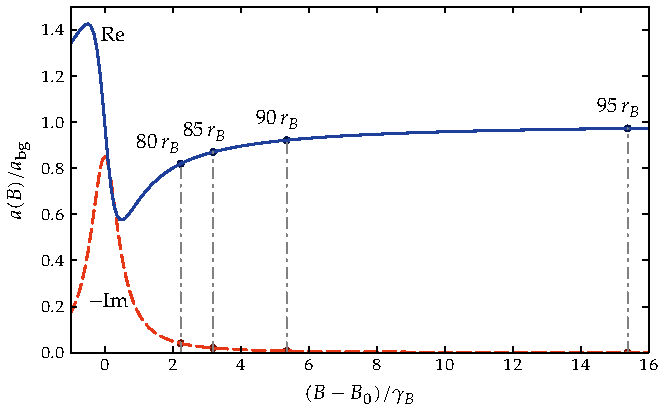
\includegraphics{figures_generated/bec_squeezing/feshbach_scattering.pdf}}

    \caption{
    Real (blue solid line) and imaginary (red dashed line, negated value is plotted for compactness) parts of the complex scattering length near the Feshbach resonance at $B_0 \approx 9.1\un{G}$.
    Four pairs of points show the distances from the resonance chosen for the demonstration, namely $0.5 \gamma_B$, $0.75 \gamma_B$, $1.0 \gamma_B$ and $1.5 \gamma_B$.
    }

    \label{fig:bec-squeezing:feshbach:scattering}
\end{figure}

For the hyperfine states we use the reported resonance parameters are $\Delta B = 9.1047\un{G}$, $\Delta B = 2\times10^{-3}\un{G}$, $\gamma_B = 4.7\times10^{-3}\un{G}$, and $a_{\mathrm{bg}} = 97.7\,r_B$.
The behavior of the real and the imaginary part of $a(B)$ near the resonance is shown in~\figref{bec-squeezing:feshbach:scattering}.
From the equations above, as well as from the figure, it is obvious that the minimum inter-species scattering length is achieved when $B - B_0 = 0.5 \gamma_B$.
Unfortunately, this value also corresponds to the relatively large value of the imaginary part, and, correspondingly, the loss rate.
Therefore, we will pick the values of $B$ further from the resonance, as displayed in the figure, where the interaction is somewhat stronger, but the loss rate is much smaller.
The equations~\eqnref{bec-squeezing:feshbach:g} and~\eqnref{bec-squeezing:feshbach:gamma} give us the following values for the simulation:
\begin{eqn}
    B - B_0 & = 2.24 \gamma_B, \quad
        a_{12} = 80.0\,r_B, \quad, \gamma_{12} = 3.85\times10^{-12}\un{cm^3/s},\\
    B - B_0 & = 2.24 \gamma_B, \quad
        a_{12} = 80.0\,r_B, \quad, \gamma_{12} = 3.85\times10^{-12}\un{cm^3/s},\\
    B - B_0 & = 2.24 \gamma_B, \quad
        a_{12} = 80.0\,r_B, \quad, \gamma_{12} = 3.85\times10^{-12}\un{cm^3/s},\\
    B - B_0 & = 2.24 \gamma_B, \quad
        a_{12} = 80.0\,r_B, \quad, \gamma_{12} = 3.85\times10^{-12}\un{cm^3/s},\\
\end{eqn}
Feshbach tuning to $a_{12} = 90.0\,a_0$ ensures the best squeezing of the four variants ($-6\un{dB}$ at $40\un{ms}$), whereas long lasting squeezing is predicted for the variant with $a_{12} = 95.0\,a_0$.

\copypaste{copypaste begins}

\begin{figure}
    \centerline{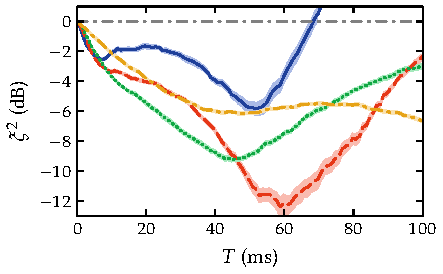
\includegraphics{figures_generated/bec_squeezing/feshbach_squeezing.pdf}}

    \caption{
    Wigner simulations of squeezing in the vicinity of $9.1\un{G}$ Feshbach resonance in \Rb.
    \todo{simulation parameters}.
    except for the inter-component scattering length and corresponding loss rate~\cite{Kaufman2009}:
    $a_{12} = 80.0\,a_0$, $\gamma^{(2)}_{12} = 3.88 \times 10^{-12}\un{cm^3/s}$ (blue solid line),
    $a_{12} = 85.0\,a_0$, $\gamma^{(2)}_{12} = 1.95 \times 10^{-12}\un{cm^3/s}$ (red dashed line),
    $a_{12} = 90.0\,a_0$, $\gamma^{(2)}_{12} = 7.13 \times 10^{-13}\un{cm^3/s}$ (green dash-dotted line) and
    $a_{12} = 95.0\,a_0$, $\gamma^{(2)}_{12} = 8.54 \times 10^{-14}\un{cm^3/s}$ (black dotted line)}

    \label{fig:bec-squeezing:feshbach:squeezing}
\end{figure}


These simulations predict the degree of quantum noise-reduction, which is a technique that can be used to improve precision quantum interferometry.
The quantum noise is initially reduced due to a stretching and rotation of the quantum noise ellipse, similar to that found in quantum soliton squeezing~\cite{Carter1987,Drummond1993a}.
For lossless environments, this effect is optimized when the cross-species scattering length is maximally different to the intra-species scattering length, which is found near the Feshbach resonance.
However, there are competing nonlinear loss effects at the Feshbach resonance, which means that some detuning of the magnetic field is essential to reduce these detrimental losses.
Subsequently, the squeezing is destroyed in time as the two fields recombine and interfere with each other.
Importantly, these quantum squeezing calculations indicate conditions that will allow this macroscopic quantum effect to be experimentally observed in ultra-cold atomic BEC for much larger atom numbers than calculated previously.

\copypaste{copypaste ends}
